\chapter{Naravna in cela števila}

 
     \section{Naravna števila}

            \textbf{Naravna števila} so števila s katerimi štejemo.
            $$\mathbf{\mathbb{N}=\{1, 2, 3, 4, \ldots\}}$$
         

          
            Množico naravnih števil definirajo \textbf{Peanovi aksiomi}:
            \begin{enumerate}
                \item Vsako naravno število $n$ ima svojega \textbf{naslednika} $n+1$.
                \item Število $1$ je naravno število, ki ni naslednik nobenega naravnega števila.
                \item Različni naravni števili imata različna naslednika: $n+1 \neq m+1; n \neq m$.
                \item Če neka trditev velja z vsakim naravnim številom tudi za njegovega naslednika, velja za vsa naravna števila. (\textit{aksiom/princip popolne indukcije})
            \end{enumerate}

         
 

 

            ~ \newline
        Naravna števila uredimo po velikosti in predstavimo s \textbf{točko} na \textbf{številski premici}.
         \begin{figure}[H]
            \centering
            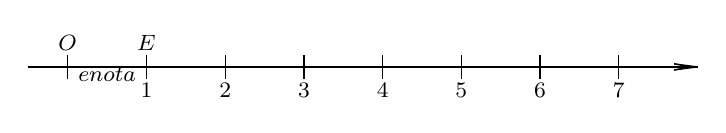
\begin{tikzpicture}
                % \clip (0,0) rectangle (14.000000,10.000000);
                {\footnotesize
                
                % Drawing segment a b
                \draw [line width=0.016cm] (0.500000,0.500000) -- (9.000000,0.500000);%
                
                % Drawing arrow a b 1.00
                \draw [line width=0.016cm] (8.702567,0.539158) -- (9.000000,0.500000);%
                \draw [line width=0.016cm] (8.702567,0.539158) -- (8.900856,0.500000);%
                \draw [line width=0.016cm] (8.702567,0.460842) -- (9.000000,0.500000);%
                \draw [line width=0.016cm] (8.702567,0.460842) -- (8.900856,0.500000);%
                
                % Drawing segment c d
                \draw [line width=0.016cm] (1.000000,0.350000) -- (1.000000,0.650000);%
                
                % Drawing segment e f
                \draw [line width=0.016cm] (2.000000,0.350000) -- (2.000000,0.650000);%
                
                % Drawing segment g h
                \draw [line width=0.016cm] (3.000000,0.350000) -- (3.000000,0.650000);%
                
                % Drawing segment i j
                \draw [line width=0.016cm] (4.000000,0.350000) -- (4.000000,0.650000);%
                
                % Drawing segment k l
                \draw [line width=0.016cm] (5.000000,0.350000) -- (5.000000,0.650000);%
                
                % Drawing segment m n
                \draw [line width=0.016cm] (6.000000,0.350000) -- (6.000000,0.650000);%
                
                % Drawing segment o p
                \draw [line width=0.016cm] (7.000000,0.350000) -- (7.000000,0.650000);%
                
                % Drawing segment r s
                \draw [line width=0.016cm] (8.000000,0.350000) -- (8.000000,0.650000);%
                
                % Marking point O
                \draw (1.000000,0.600000) node [anchor=south] { $O$ };%
                
                % Marking point E
                \draw (2.000000,0.600000) node [anchor=south] { $E$ };%
                
                % Marking point 1
                \draw (2.000000,0.400000) node [anchor=north] { $1$ };%
                
                % Marking point 2
                \draw (3.000000,0.400000) node [anchor=north] { $2$ };%
                
                % Marking point 3
                \draw (4.000000,0.400000) node [anchor=north] { $3$ };%
                
                % Marking point 4
                \draw (5.000000,0.400000) node [anchor=north] { $4$ };%
                
                % Marking point 5
                \draw (6.000000,0.400000) node [anchor=north] { $5$ };%
                
                % Marking point 6
                \draw (7.000000,0.400000) node [anchor=north] { $6$ };%
                
                % Marking point 7
                \draw (8.000000,0.400000) node [anchor=north] { $7$ };%
                
                % Marking point {enota}
                \draw (1.500000,0.600000) node [anchor=north] { ${enota}$ };%
                }
            \end{tikzpicture}
                
        \end{figure}

     

      
        Vsako število zapišemo s \textbf{številko}. 
        Za zapis številke uporabljamo \textbf{števke}. Te so $0, 1, 2, 3, 4, 5, 6, 7, 8, 9$.
     

      
        Posamezne števke večmestnega števila od desne proti levi predstavljajo: \textbf{enice}, \textbf{desetice}, \textbf{stotice}, \textbf{tisočice}, ...
     

        ~\newline
        Število, ki je zapisano s črkovnimi oznakami števk označimo s črto nad zapsiom črkovne oznake.
        $$ \overline{xy}=10x+y \quad \quad \quad \overline{xyz}=100x+10y+z$$
     

    
 

 
     \section{Operacije v množici $\mathbb{N}$}

     \subsection{Seštevanje}
        Poljubnima naravnima številoma $x$ in $y$ priredimo \textbf{vsoto} $\mathbf{x+y}$.
        \newline

        Število $x$ oziroma $y$ imenujemo \textbf{seštevanec} ali \textbf{sumand} ali \textbf{člen}. 
        Število $x+y$ pa imenujemo \textbf{vsota} ali \textbf{summa}. 

     \begin{figure}[H]
        \centering

        \begin{tikzpicture}
            % \clip (0,0) rectangle (14.000000,10.000000);
            {\footnotesize
            
            % Drawing segment a b
            \draw [line width=0.016cm] (5.000000,0.500000) -- (5.000000,2.500000);%
            
            % Drawing segment b d
            \draw [line width=0.016cm] (5.000000,2.500000) -- (7.000000,2.500000);%
            
            % Drawing segment c d
            \draw [line width=0.016cm] (7.000000,0.500000) -- (7.000000,2.500000);%
            
            % Drawing segment c a
            \draw [line width=0.016cm] (7.000000,0.500000) -- (5.000000,0.500000);%
            
            % Drawing segment e f
            \draw [line width=0.016cm] (7.000000,1.500000) -- (9.000000,1.500000);%
            
            % Drawing arrow e f 1.00
            \draw [line width=0.016cm] (8.702567,1.539158) -- (9.000000,1.500000);%
            \draw [line width=0.016cm] (8.702567,1.539158) -- (8.900856,1.500000);%
            \draw [line width=0.016cm] (8.702567,1.460842) -- (9.000000,1.500000);%
            \draw [line width=0.016cm] (8.702567,1.460842) -- (8.900856,1.500000);%
            
            % Drawing segment g h
            \draw [line width=0.016cm] (2.500000,1.000000) -- (5.000000,1.000000);%
            
            % Drawing segment i j
            \draw [line width=0.016cm] (2.500000,2.000000) -- (5.000000,2.000000);%
            
            % Drawing arrow g h 1.00
            \draw [line width=0.016cm] (4.702567,1.039158) -- (5.000000,1.000000);%
            \draw [line width=0.016cm] (4.702567,1.039158) -- (4.900856,1.000000);%
            \draw [line width=0.016cm] (4.702567,0.960842) -- (5.000000,1.000000);%
            \draw [line width=0.016cm] (4.702567,0.960842) -- (4.900856,1.000000);%
            
            % Drawing arrow i j 1.00
            \draw [line width=0.016cm] (4.702567,2.039158) -- (5.000000,2.000000);%
            \draw [line width=0.016cm] (4.702567,2.039158) -- (4.900856,2.000000);%
            \draw [line width=0.016cm] (4.702567,1.960842) -- (5.000000,2.000000);%
            \draw [line width=0.016cm] (4.702567,1.960842) -- (4.900856,2.000000);%
            
            % Marking point {vsota}
            \draw (8.000000,1.500000) node [anchor=south] { ${vsota}$ };%
            
            % Marking point {summa}
            \draw (8.000000,1.500000) node [anchor=north] { ${summa}$ };%
            
            % Marking point {se�tevanec}
            \draw (3.750000,1.000000) node [anchor=south] { ${seštevanec}$ };%
            
            % Marking point {sumand}
            \draw (3.750000,1.000000) node [anchor=north] { ${sumand}$ };%
            
            % Marking point {se�tevanec}
            \draw (3.750000,2.000000) node [anchor=south] { ${seštevanec}$ };%
            
            % Marking point {sumand}
            \draw (3.750000,2.000000) node [anchor=north] { ${sumand}$ };%
            
            % Drawing segment x y
            \draw [line width=0.032cm] (6.000000,1.000000) -- (6.000000,2.000000);%
            
            % Drawing segment z w
            \draw [line width=0.032cm] (5.500000,1.500000) -- (6.500000,1.500000);%
            }
            \end{tikzpicture}
            
    \end{figure}


     


      
        Vsota naravnih števil je naravno število: $x, y \in \mathbb{N} \Rightarrow x+y \in \mathbb{N}$.

     

 

 
     \subsection{Množenje}
        Poljubnima naravnima številoma $x$ in $y$ priredimo \textbf{produkt} $\mathbf{x\cdot y}$.
        \newline

        Število $x$ oziroma $y$ imenujemo \textbf{množenec} ali \textbf{faktor}. 
        Število $x\cdot y$ pa imenujemo \textbf{zmnožek} ali \textbf{produkt}. 

         \begin{figure}[H]
            \centering

        \begin{tikzpicture}
            % \clip (0,0) rectangle (14.000000,10.000000);
            {\footnotesize
            
            % Drawing segment a b
            \draw [line width=0.016cm] (5.000000,0.500000) -- (5.000000,2.500000);%
            
            % Drawing segment b d
            \draw [line width=0.016cm] (5.000000,2.500000) -- (7.000000,2.500000);%
            
            % Drawing segment c d
            \draw [line width=0.016cm] (7.000000,0.500000) -- (7.000000,2.500000);%
            
            % Drawing segment c a
            \draw [line width=0.016cm] (7.000000,0.500000) -- (5.000000,0.500000);%
            
            % Drawing segment e f
            \draw [line width=0.016cm] (7.000000,1.500000) -- (9.000000,1.500000);%
            
            % Drawing arrow e f 1.00
            \draw [line width=0.016cm] (8.702567,1.539158) -- (9.000000,1.500000);%
            \draw [line width=0.016cm] (8.702567,1.539158) -- (8.900856,1.500000);%
            \draw [line width=0.016cm] (8.702567,1.460842) -- (9.000000,1.500000);%
            \draw [line width=0.016cm] (8.702567,1.460842) -- (8.900856,1.500000);%
            
            % Drawing segment g h
            \draw [line width=0.016cm] (2.500000,1.000000) -- (5.000000,1.000000);%
            
            % Drawing segment i j
            \draw [line width=0.016cm] (2.500000,2.000000) -- (5.000000,2.000000);%
            
            % Drawing arrow g h 1.00
            \draw [line width=0.016cm] (4.702567,1.039158) -- (5.000000,1.000000);%
            \draw [line width=0.016cm] (4.702567,1.039158) -- (4.900856,1.000000);%
            \draw [line width=0.016cm] (4.702567,0.960842) -- (5.000000,1.000000);%
            \draw [line width=0.016cm] (4.702567,0.960842) -- (4.900856,1.000000);%
            
            % Drawing arrow i j 1.00
            \draw [line width=0.016cm] (4.702567,2.039158) -- (5.000000,2.000000);%
            \draw [line width=0.016cm] (4.702567,2.039158) -- (4.900856,2.000000);%
            \draw [line width=0.016cm] (4.702567,1.960842) -- (5.000000,2.000000);%
            \draw [line width=0.016cm] (4.702567,1.960842) -- (4.900856,2.000000);%
            
            % Marking point {zmno�ek}
            \draw (8.000000,1.500000) node [anchor=south] { ${zmnožek}$ };%
            
            % Marking point {produkt}
            \draw (8.000000,1.500000) node [anchor=north] { ${produkt}$ };%
            
            % Marking point {mno�enec}
            \draw (3.750000,1.000000) node [anchor=south] { ${množenec}$ };%
            
            % Marking point {faktor}
            \draw (3.750000,1.000000) node [anchor=north] { ${faktor}$ };%
            
            % Marking point {mno�enec}
            \draw (3.750000,2.000000) node [anchor=south] { ${množenec}$ };%
            
            % Marking point {faktor}
            \draw (3.750000,2.000000) node [anchor=north] { ${faktor}$ };%
            
            % Drawing circle k
            \draw [line width=0.016cm] (6.000000,1.500000) circle (0.100000);%
            
            % Filling circle k
            \fill (6.000000,1.500000) circle (0.100000);%
            }
            \end{tikzpicture}
            
    \end{figure}

     
        Produkt naravnih števil je naravno število: $x, y \in \mathbb{N} \Rightarrow x\cdot y \in \mathbb{N}$.
        \newline

        Število $\mathbf{1}$ je \textbf{nevtralni element} za mmnoženje: $1\cdot x = x$.
     \newline

 
        Seštevanje in množenje sta \textit{dvočleni notranji operaciji} v množici naravnih števil $\mathbb{N}$.

 
    

     \subsection{Odštevanje}
        Številoma $x$ in $y$, pri čemer je $y$ večje od $x$ ($x>y$), priredimo \textbf{razliko} $\mathbf{x-y}$.                
        \newline

        Število $x$ imenujemo \textbf{zmanjševanec} ali \textbf{minuend}, število $y$  pa imenujemo \textbf{odštevanec} ali \textbf{subtrahend}. 
        Številu $x-y$ rečemo \textbf{razlika} ali \textbf{diferenca}. 

         \begin{figure}[H]
            \centering
            \begin{tikzpicture}
                % \clip (0,0) rectangle (14.000000,10.000000);
                {\footnotesize
                
                % Drawing segment a b
                \draw [line width=0.016cm] (5.000000,0.500000) -- (5.000000,2.500000);%
                
                % Drawing segment b d
                \draw [line width=0.016cm] (5.000000,2.500000) -- (7.000000,2.500000);%
                
                % Drawing segment c d
                \draw [line width=0.016cm] (7.000000,0.500000) -- (7.000000,2.500000);%
                
                % Drawing segment c a
                \draw [line width=0.016cm] (7.000000,0.500000) -- (5.000000,0.500000);%
                
                % Drawing segment e f
                \draw [line width=0.016cm] (7.000000,1.500000) -- (9.000000,1.500000);%
                
                % Drawing arrow e f 1.00
                \draw [line width=0.016cm] (8.702567,1.539158) -- (9.000000,1.500000);%
                \draw [line width=0.016cm] (8.702567,1.539158) -- (8.900856,1.500000);%
                \draw [line width=0.016cm] (8.702567,1.460842) -- (9.000000,1.500000);%
                \draw [line width=0.016cm] (8.702567,1.460842) -- (8.900856,1.500000);%
                
                % Drawing segment g h
                \draw [line width=0.016cm] (2.500000,1.000000) -- (5.000000,1.000000);%
                
                % Drawing segment i j
                \draw [line width=0.016cm] (2.500000,2.000000) -- (5.000000,2.000000);%
                
                % Drawing arrow g h 1.00
                \draw [line width=0.016cm] (4.702567,1.039158) -- (5.000000,1.000000);%
                \draw [line width=0.016cm] (4.702567,1.039158) -- (4.900856,1.000000);%
                \draw [line width=0.016cm] (4.702567,0.960842) -- (5.000000,1.000000);%
                \draw [line width=0.016cm] (4.702567,0.960842) -- (4.900856,1.000000);%
                
                % Drawing arrow i j 1.00
                \draw [line width=0.016cm] (4.702567,2.039158) -- (5.000000,2.000000);%
                \draw [line width=0.016cm] (4.702567,2.039158) -- (4.900856,2.000000);%
                \draw [line width=0.016cm] (4.702567,1.960842) -- (5.000000,2.000000);%
                \draw [line width=0.016cm] (4.702567,1.960842) -- (4.900856,2.000000);%
                
                % Marking point {razlika}
                \draw (8.000000,1.500000) node [anchor=south] { ${razlika}$ };%
                
                % Marking point {diferenca}
                \draw (8.000000,1.500000) node [anchor=north] { ${diferenca}$ };%
                
                % Marking point {od�tevanec}
                \draw (3.750000,1.000000) node [anchor=south] { ${odštevanec}$ };%
                
                % Marking point {subtrahend}
                \draw (3.750000,1.000000) node [anchor=north] { ${subtrahend}$ };%
                
                % Marking point {zmanj�evanec}
                \draw (3.750000,2.000000) node [anchor=south] { ${zmanjševanec}$ };%
                
                % Marking point {minuend}
                \draw (3.750000,2.000000) node [anchor=north] { ${minuend}$ };%
                
                % Drawing segment z w
                \draw [line width=0.032cm] (5.500000,1.500000) -- (6.500000,1.500000);%
                }
                \end{tikzpicture}
                
    \end{figure}
 

      
        Razlika je število, ki ga moramo prišteti številu $y$, da dobimo število $y$.
        $$ (x-y)+y=x $$


        Odštevanje ni notranja operacija v množici naravnih števil $\mathbb{N}$.
     

     \subsection{Vrstni red operacij}
        Prednost pri računanju imajo \textbf{oklepaji} (najprej najbolj notranji), nato sledi \textbf{množenje},
        na koncu pa imamo še \textbf{seštevanje} in \textbf{odštevanje}.
     

      
        Kadar v izrazu nastopajo enakovredne računske operacije, računamo od leve proti desni.
     

        ~\newline

        Pri množenju količin, ki so označene s črkovnimi oznakami, piko, ki označuje operacijo množenja ponavadi opustimo.
        $$ x\cdot y = xy$$
     


 

 
     \section{Osnovni računski zakoni}

     \subsection*{Komutativnost seštevanja -- zakon o zamenjavi členov}
        $$ \mathbf{x+y=y+x}$$
        Vsota ni odvisna od vrstnega reda seštevanja.
     

        \subsection*{Asociativnost seštevanja -- zakon o poljubnem združevanju členov}
        $$ \mathbf{(x+y)+z=x+(y+z)}$$
        Vsota več kot dveh sumandov ni odvisna od združevanja po dveh sumandov.
     

        \subsection*{Komutativnost množenja -- zakon o zamenjavi faktorjev}
        $$ \mathbf{x\cdot y=y\cdot x}$$
        Produkt ni odvisna od vrstnega reda faktorjev.
     

        \subsection*{Asociativnost množenja -- zakon o poljubnem združevanju faktorjev}
        $$ \mathbf{(x\cdot y)\cdot z=x\cdot (y\cdot z)}$$
        Produkt več kot dveh sumandov ni odvisen od združevanja faktorjev.
     
        \subsection*{Distributivnost -- zakon o razčlenjevanju}
        $$ \mathbf{x\cdot z+y\cdot z = (x+y)\cdot z} $$
        Če to beremo iz desne proti levi, rečemu tudi \textit{pravilo izpostavljanja skupnega faktorja}.
        \newline ~
        \newline
 

 
     \begin{naloga}
        Izračunajte.
        \begin{itemize}
            \item $(1+2\cdot 7)+3\cdot(2\cdot 2+7)$ 
            \item $3\cdot(2+3\cdot 5)\cdot(2+1)$ 
            \item $7+(2+6\cdot 3)+(8+4\cdot 5)$ 
            \item $11\cdot 4+(12-6)\cdot 5$ 
            \item $8+2\cdot(3+7)-15$ 
            \item $37-5\cdot(10-3)$ 
        \end{itemize}
     \end{naloga}
 

 
     \begin{naloga}
        Hitro izračunajte.
        \begin{itemize}
            \item $45+37+15$ 
            \item $108+46-28$
            \item $5\cdot 13\cdot 8$
            \item $4\cdot 7\cdot 25$
            \item $(7+3)\cdot 2\cdot 5$
            \item $15\cdot(4+6)\cdot 2$
            \item $3\cdot 5+7\cdot 5$
            \item $8\cdot 12+6\cdot 8$
        \end{itemize}
     \end{naloga}
 

 
     \begin{naloga}
        Zapišite račun glede na besedilo in izračunajte.
        \begin{itemize}
            \item Produktu števil $12$ in $27$ odštejte razliko števil $19$ in $11$. 
            \item Vsoti produkta $4$ in $12$ ter produkta $5$ in $16$ odštejte $8$. 
            \item Vsoto števil $42$ in $23$ pomnožite z razliko števil $58$ in $29$. 
            \item Produkt števil $14$ in $17$ pomnožite z vsoto števil $5$ in $16$. 
        \end{itemize}
     \end{naloga}
 

 
     \begin{naloga}
        Rešite besedilno nalogo.
        \begin{itemize}
            \item V trgovini kupimo tri litre mleka in štiri čokoladne pudinge v prahu. Če stane liter mleka $95$ centov,
                čokoladni puding v prahu pa $24$ centov, koliko moramo plačati? 
            \item Manca bo kuhala rižoto za štiri otroke in šest odraslih. Za otroško porcijo rižote zadošča $45~g$ riža,
                za odraslo pa $75~g$. Koliko riža mora dati kuhati za rižoto? 
        \end{itemize}
     \end{naloga}
 


\newpage
   \section{Cela Števila}
         
                    $$\mathbf{\mathbb{Z} = \{\ldots, -2, -1, 0, 1, 2, 3, \ldots\}}$$
                

                 
                    Množica celih števil $\mathbb{Z}$ je definirana kot unija treh množic:
                        \begin{itemize}
                            \item množica \textbf{pozitivnih celih števil} ($\mathbb{Z}^+$) -- naravna števila $\mathbb{N}$;
                            \item \textbf{število 0};
                            \item množica \textbf{negativnih celih števil} ($\mathbb{Z}^-$) -- nasprotna števila vseh naravnih števil.
                        \end{itemize}
                      $$\mathbb{Z} = \mathbb{Z}^- \cup \{0\} \cup \mathbb{Z}^+$$

                 

                 
                    \textbf{Nasprotna vrednost} števila $n$ je število $-n$.
                 
         

         
             \section{Operacije v množici $\mathbb{Z}$}

            \subsection{Seštevanje}

             
                $$\mathbf{x+0=x}; ~\forall x\in\mathbb{Z}$$
                Število $0$ je \textbf{nevtralni element} pri seštevanju.
             

             
                $$\mathbf{x+(-x)=0}; ~\forall x\in\mathbb{Z} $$
                Vsota celega števila in njemu nasprotnega števila je enaka $0$.
             

             
                $$\mathbf{-(-x)=x}; ~\forall x\in\mathbb{Z}$$
                Nasprotna vrednost nasprotne vrednosti je enaka prvotni vrednosti.
             \newline
         

             
                Vsota dveh pozitivnih števil je pozitivno število, vsota dveh negativnih števil pa je negativno število.
             

             
                $$\mathbf{-x+(-y)=-(x+y)}$$
                Vsota nasprotnih vrednosti je enaka nasprotni vrednosti vsote.
             \newline

             
                Naj bosta $x$ in $y$ naravni števili. Vsota pozitivnega števila $x$ in negativnega števila $-y$ je:
                \begin{itemize}
                    \item pozitivno število, če je $x>y$ in
                    \item negativno število, če je $x<y$.
                \end{itemize}
             
         


         
            \subsection{Odštevanje}

             
                Razlika $x-y$ dveh pozitivnih števil $x$ in $y$ je:
                \begin{itemize}
                    \item pozitivno število, če je $x>y$ in 
                    \item negativno število, če je $x<y$.
                \end{itemize}
               ~

             
                Razlika dveh negativnih števil $(-x)-(-y)$ je:
                \begin{itemize}
                    \item pozitvno število, če je $x<y$ in 
                    \item negativno število, če je $x>y$.
                \end{itemize}
               ~

             
                Razlika pozitivnega števila $x$ in negativnega števila $-y$ je pozitvno število.
                ~\newline


            
                \textit{Odštevanje v množici $\mathbb{Z}$ je prištevanje nasprotne vrednosti.}
                $$\mathbf{x-y=x+(-y)} $$
            
         

         
            \subsection{Množenje}

             
                $$\mathbf{1\cdot x=x}; ~\forall x\in\mathbb{Z}$$
                Število $1$ je \textbf{nevtralni element} za množenje.
             

             
                $$\mathbf{(-1)\cdot x=-x}; ~\forall x\in\mathbb{Z}$$
                Pri množenju celega števila $x$ z $-1$ dobimo nasprotno število $-x$.
             

             
                $$\mathbf{0\cdot x=0}; ~\forall x\in\mathbb{Z}$$
                Rezultat množenja števila s številom $0$ je enak $0$.
             

         

         


             
                $$\mathbf{(-x)(-y)=xy}$$
                Produkt sodo mnogo negativnih števil je pozitivno število.
             

             
                $$\mathbf{-x\cdot y=-(xy)}$$
                $$\mathbf{x(-y)=-(xy)}$$
                Produkt pozitivnega in negativnega števila je negativno število.
             

             
                $$\mathbf{(-x)(-y)=xy}$$
                Produkt liho mnogo negativnih faktorjev je negativno število.
                ~\newline

             
                Seštevanje, odštevanje in množenje so v množici $\mathbb{Z}$ dvočlene notranje operacije.
             
         
                
                    \section{Osnovni računski zakoni v $\mathbb{Z}$}



                    \subsection*{Komutativnost seštevanja}
                    $$ \mathbf{x+y=y+x}$$
                    Vsota ni odvisna od vrstnega reda seštevanja.
                 
            
                    \subsection*{Asociativnost seštevanja}
                    $$ \mathbf{(x+y)+z=x+(y+z)}$$
                    Vsota več kot dveh sumandov ni odvisna od združevanja po dveh sumandov.
                 
            
                    \subsection*{Komutativnost množenja}
                    $$ \mathbf{x\cdot y=y\cdot x}$$
                    Produkt ni odvisna od vrstnega reda faktorjev.
                 
            
                    \subsection*{Asociativnost množenja}
                    $$ \mathbf{(x\cdot y)\cdot z=x\cdot (y\cdot z)}$$
                    Produkt več kot dveh sumandov ni odvisen od združevanja faktorjev.
                 
                    \subsection*{Distributivnost seštevanja in množenja ter odštevanja in množenja}
                    $$ \mathbf{x\cdot z+y\cdot z = (x+y)\cdot z} $$
                    $$ \mathbf{x\cdot z-y\cdot z = (x-y)\cdot z} $$

                    Če to beremo iz desne proti levi, rečemu tudi \textit{pravilo izpostavljanja skupnega faktorja}.
            
        
                
                    \begin{naloga}
                        Izračunajte.
                        \begin{itemize}
                            \item $17-13-2+10$  
                            \item $50+11-32-14$  
                            \item $3+((5+2(7-9))\cdot 2-1)$  
                            \item $(2-5(6-10))\cdot(5-2(7-5))$  
                            \item $9(11-3)+7(10-15)$  
                            \item $8+9(11-18)-2\cdot 5$  
                        \end{itemize}
                    \end{naloga}
                
                    \begin{naloga}
                        Spretno izračunajte.
                        \begin{itemize}
                            \item $7\cdot 8-12\cdot 8$  
                            \item $5\cdot 18+9\cdot 5-5\cdot 2$  
                            \item $8\cdot(4-9)\cdot 2$  
                            \item $5\cdot 3\cdot (12-8)$  
                            \item $(15-6)(12-3\cdot 4)$  
                        \end{itemize}
                    \end{naloga}
                
                    \begin{naloga}
                        Rešite besedilne naloge.
                        \begin{itemize}
                            \item V hotelu imajo na voljo osemnajst enoposteljnih, štiriintrideset dvoposteljnih in petindevetdeset triposteljnih sob.
                                Koliko ljudi lahko še prespi v hotelu, če je v njem že sto triinštirideset gostov?      
                            \item Pohod na bližnji hrib traja tri ure. Koliko minut moramo še hoditi, če smo na poti že $145$ minut?       
                            \item S Ptuja in iz Postojne (razdalja med njima je približno $190~km$) sočasno odpeljeta dva motorista drug proti drugemu.
                                En vozi povprečno $40~km/h$, drugi pa $5~km/h$ manj. Kolikšna bo razdalja med njima po dveh urah vožnje?      
                        \end{itemize}
                    \end{naloga}
        
                    \begin{naloga}
                        Zapišite enačbe in jih poenostavite.
                        \begin{itemize}
                            \item Razlika petkratnka $a$ in $b$ je enaka trikratniku vsote štirikratnika $a$ in petkratnika $b$.   
                            \item Vsota $x$ in dvakratnika $y$ je enaka razliki petkratnika $x$ in dvanajstkratnika $y$.    
                        \end{itemize}
                    \end{naloga}


                    
\newpage
\section{Urejenost naravnih in celih števil}


    
        Številska množica je \textbf{urejena}, kadar lahko po velikosti primerjamo njena poljubna elementa.
    

    
        Pri urejanju števil uporabljamo naslednje znake:
        \begin{table}[H]
            \centering
            \addtolength{\tabcolsep}{6pt}
            \renewcommand{\arraystretch}{1.4}                
            \begin{tabular}{||c|c||} 
                \hhline{|t:==:t|}
                        $\mathbf{<}$ & manjše / manj  \\ 
                \hline
                        $\mathbf{>}$ & večje / več   \\ 
                \hline
                        $\mathbf{\leq}$ & manjše ali enako / največ   \\ 
                \hline
                        $\mathbf{\geq}$ & večje ali enako / vsaj, najmanj \\  
                \hline
                        $\mathbf{=}$ & enako \\
                \hhline{|b:==:b|}
            \end{tabular}
        \end{table}
    



    
        Za poljubni števili $x,y\in\mathbb{Z}$ velja natanko ena izmed naslednjih možnosti: $x>y$, $x<y$ ali $x=y$.
    \newline

            Slika števila $x$ leži na številski premici desno od slike števila $y$:
        $$\mathbf{x>y \Leftrightarrow x-y>0}$$
    

            Slika števila $x$ leži na številski premici levo od slike števila $y$:
        $$\mathbf{x<y \Leftrightarrow x-y<0}$$
    

            Slika števila $x$ sovpada s sliko števila $y$:
        $$\mathbf{x=y \Leftrightarrow x-y=0}$$
    \newline

    
        Velja pa tudi:
        $$x\leq y \Leftrightarrow x-y\leq 0 $$
        $$x\geq y \Leftrightarrow x-y\geq 0 $$


    \subsubsection*{Pozitivna in negativna števila}
        V množici $\mathbb{Z}$ so pozitivna tista števila, ki so večja od števila $0$ 
        in njihove slike ležijo desno od izhodišča, 
        negativna pa tista števila, ki so manjša od števila $0$ 
        in njihove slike ležijo levo od izhodišča.
    
        Vsako pozitivno celo število (vsako naravno število) je večje od katerega koli negativnega celega števila.
    



    


        \subsection{Linearna urejenost}

    
        Z relacijo \textit{biti manjši ali enak} je množica $\mathbb{Z}$ \textbf{linearno urejena}, 
        to pomeni, da veljajo naslednje lastnosti: refleksivnost, antisimetričnost, tranzitivnost, stroga sovisnost.
    
    
        \subsubsection*{Refleksivnost}
        $$\forall x\in\mathbb{Z}: x\leq x$$
    

        \subsubsection*{Antisimetričnost}
        $$\forall x,y\in\mathbb{Z}: x\leq y \land y\leq x \Rightarrow x=y$$
    

        \subsubsection*{Tranzitivnost}
        $$\forall x,y,z\in\mathbb{Z}: x\leq y \land y\leq z \Rightarrow x\leq z$$
    

        \subsubsection*{Stroga sovisnost}
        $$\forall x,y\in\mathbb{Z}; x\neq y: x\leq y \lor y\leq x$$

    



        \subsection{Lastnosti relacij $\leq$ in $<$}
        \subsubsection*{Monotonost vsote}
        $$x<y \Rightarrow x+z<y+z \quad \quad x\leq y \Rightarrow x+z\leq y+z$$
        Če na obeh straneh neenakosti prištejemo isto število, se neenakost ohrani.
    \newline

    
        $$x<y \land z>0 \Rightarrow x\cdot z<y\cdot z \quad \quad x\leq y \land z>0 \Rightarrow x\cdot z\leq y\cdot z$$
        Pri množenju neenakosti z negativnim številom se znak neenakosti ohrani.
        \newline

    
        $$x<y \land z<0 \Rightarrow x\cdot z>y\cdot z \quad \quad x\leq y \land z<0 \Rightarrow x\cdot z\geq y\cdot z$$
        Pri množenju neenakosti z negativnim številom se znak neenakosti obrne.
        \newline ~
        \newline

    
        Obravnavane lastnosti veljajo tudi za relaciji $\geq$ in $>$.
        \newline ~
        \newline ~
        \newline





        \begin{naloga}
            Uredite števila $3, -2, 5, -1, 0, -7, 6, -6$ po velikosti in jih predstavite na številski premici.
        \end{naloga}

        \begin{naloga}
            Uredite števila $104, -27, 35, -107, 36, -26, 25, -28, 81$ po velikosti.
        \end{naloga}

        \begin{naloga}
            Gladina Mrtvega morja leži v depresiji na $-423~m$ nadmorske višine, njegova največja globina pa je $378~m$.
            Kolikšna je najmanjša nadmorska višina dna Mrtvega morja?
        \end{naloga}

        \begin{naloga}
            Za katera cela števila $x$ ima izraz $3x-5(x+2)$ večjo ali enako vrednost od izraza $4-(12+x)$?
        \end{naloga}



